%\documentclass[sigplan,screen,authordraft]{acmart}
\documentclass[sigplan,anonymous,review]{acmart}
%%
%% \BibTeX command to typeset BibTeX logo in the docs
\AtBeginDocument{%
  \providecommand\BibTeX{{%
    \normalfont B\kern-0.5em{\scshape i\kern-0.25em b}\kern-0.8em\TeX}}}

%% Rights management information.  This information is sent to you
%% when you complete the rights form.  These commands have SAMPLE
%% values in them; it is your responsibility as an author to replace
%% the commands and values with those provided to you when you
%% complete the rights form.

\setcopyright{acmcopyright}
\copyrightyear{2018}
\acmYear{2018}
\acmDOI{10.1145/1122445.1122456}

%GPCE 2021 - 20th International Conference on Generative Programming: Concepts & Experiences

%\acmConference[Woodstock '18]{Woodstock '18: ACM Symposium on Neural
%  Gaze Detection}{June 03--05, 2018}{Woodstock, NY}
%\acmBooktitle{Woodstock '18: ACM Symposium on Neural Gaze Detection,
%  June 03--05, 2018, Woodstock, NY}
%\acmPrice{15.00}
%\acmISBN{978-1-4503-XXXX-X/18/06}




\begin{document}

%Title suggestions
\title{Towards a Declarative Framework for Machine Learning}
\subtitle{Short Paper}
%\titlenote{Short Paper}
% \title{COPPE: EDSL, Haskell and deep learning stuff}
%\title{A Declarative Framework for Analysis of Machine Learning Algorithms}


\author{Bo Joel Svensson}
\affiliation{%
  \institution{Chalmers University of Technology}
  \city{Gothenburg}
  \country{Sweden}
} 
\email{bo.joel.svensson@gmail.com}
\author{Yinan Yu}
\affiliation{%
  \institution{Chalmers University of Technology}
  \city{Gothenburg}
  \country{Sweden}}
\email{yu.yinan16@gmail.com}
\author{Mary Sheeran}
\affiliation{%
  \institution{Chalmers University of Technology}
  \city{Gothenburg}
  \country{Sweden}}
\email{mary.sheeran@chalmers.se}

\renewcommand{\shortauthors}{Svensson, et al.}

\begin{abstract}

  abstracty stuff

\end{abstract}

%%
%% The code below is generated by the tool at http://dl.acm.org/ccs.cfm.
%% Please copy and paste the code instead of the example below.
%%
\begin{CCSXML}
<ccs2012>
 <concept>
  <concept_id>10010520.10010553.10010562</concept_id>
  <concept_desc>Computer systems organization~Embedded systems</concept_desc>
  <concept_significance>500</concept_significance>
 </concept>
 <concept>
  <concept_id>10010520.10010575.10010755</concept_id>
  <concept_desc>Computer systems organization~Redundancy</concept_desc>
  <concept_significance>300</concept_significance>
 </concept>
 <concept>
  <concept_id>10010520.10010553.10010554</concept_id>
  <concept_desc>Computer systems organization~Robotics</concept_desc>
  <concept_significance>100</concept_significance>
 </concept>
 <concept>
  <concept_id>10003033.10003083.10003095</concept_id>
  <concept_desc>Networks~Network reliability</concept_desc>
  <concept_significance>100</concept_significance>
 </concept>
</ccs2012>
\end{CCSXML}

\ccsdesc[500]{Computer systems organization~Embedded systems}
\ccsdesc[300]{Computer systems organization~Redundancy}
\ccsdesc{Computer systems organization~Robotics}
\ccsdesc[100]{Networks~Network reliability}

\keywords{neural networks}

%% A "teaser" image appears between the author and affiliation
%% information and the body of the document, and typically spans the
%% page.
%% \begin{teaserfigure}
%%   \includegraphics[width=\textwidth]{sampleteaser}
%%   \caption{Seattle Mariners at Spring Training, 2010.}
%%   \Description{Enjoying the baseball game from the third-base
%%   seats. Ichiro Suzuki preparing to bat.}
%%   \label{fig:teaser}
%% \end{teaserfigure}

\maketitle


% PLAN: (May 14)
%
% Description of Coppe
%   - How we model deep learning
%   - Easy to analyse
%   - Yaml interfaces/EDSL interface (Monad, Arrow)
%
% EDSL Programming example.
%   - Digit recognition? (find tutorial, generate the same code)
%
% Generate python *
%   - It is not hard to argue that deep learning code is full of errors
%   - Show that our approach is less full of errors.
%   - Maybe proof of concept
%
% Case study
%   - Look at some
%
% Evaluation
%   - What can we show?
%   - What kind of errors are users making
%     - Example error -> coppe helps avoid/correct it.
%
% Future work
%   - Speed / memory
%   - Database
%   - Vanishing gradient
%   -

\section{Introduction}

Introductory stuff

\section{Motivation}


Deep learning is a family of data driven techniques that have been applied in various professional domains, such as medical diagnostics, autonomous driving, drug discovery and many more.
The purpose of these techniques is to help human actors make better decisions from observing a large amount of data.

On an abstract level, given input data $x$, deep learning models can be expressed as $f(x; w)$, where $f$ is a function of $x$ and $w$ refers to unknown parameters in the model, which are then inferred from data. This is why deep learning is called \emph{data driven}: a large proportion of the mathematical expression $f$ is inferred from and hence determined by data.

There are two main steps in deep learning: \emph{training} and \emph{inference}.
\emph{Training} is the process where the unknown parameters $w$ are being derived from a given set of data in an iterative manner and \emph{inference} is the application of the function $f$ given these inferred $w$. Because of the potentially large number of unknown parameters and the highly complex form of $f$, the training process can take a very long time to complete.

Data driven approaches can be very powerful. They apply patterns that go beyond human knowledge and experience. However, the downside is that these techniques are hard to verify, interpret and reproduce.

If we take one step back and further break down the construction of a deep learning program, it usually goes like this:
\begin{itemize}
\item {\bf Step 1}: construct $f(\cdot; w\mid h)$. This step is sometimes called the \emph{first selection problem} or \emph{model selection} in machine learning. There are three parts in constructing this function: 1) the general form of the mathematical expression $f$, 2) \emph{hyperparameters} $h$ and 3) the unknown parameters $w$. The unknown parameters will be inferred from data automatically at a later stage, but as the developer, one needs to first manually choose 1) and 2). The hyperparameters $h$ refer to a set of parameters that can be changed to modify the form of the function.
  Unlike the unknown parameters $w$, the hyperparameters are typically determined by human developers. For that reason, we write $h$ on the right side of the vertical bar $\mid$ to indicate that it is a set of \emph{given} values.
  There are two sub-steps in this process:
  \begin{itemize}
  \item {\bf Step 1.1}: choose $f$ and $h$ based on theories, experience and human intuition
  \item {\bf Step 1.2}: implement the deep learning model as a computer program
  \end{itemize}
\item {\bf Step 2}: derive the unknown parameters $w$ from a set of data $\mathcal{X}_0$. This step is referred to as the \emph{second selection problem} or \emph{training} in machine learning. For this reason, $w$ is usually called the \emph{trainable parameters}. This is an automatic process typically implemented by backpropagation. Here we use $\hat{w}$ to denote the estimates of the unknown parameters $w$.
\item {\bf Step 3}: evaluate the model $f(\cdot; \hat{w}\mid h)$ on a separate data set $\mathcal{X}_1$ by applying the function $f(x; \hat{w}\mid h), \forall x\in\mathcal{X}_1$ and compare the results to the ground truth. This step is to validate the choice of $f$ and $h$ by evaluating the quality of $\hat{w}$. Note that since $\hat{w}$ is derived from $\mathcal{X}_0$, the validation has to be based on a different set of data $\mathcal{X}_1$.
\item Iterate from step 1 until a desirable outcome is achieved by step 3.
\end{itemize}

\paragraph{What could possibly go wrong?}
At a first glance, the process seems well established. However, there are a couple of challenges when it comes to deep learning.
\begin{itemize}
\item Step 1.1: it is difficult to choose and keep track of $f$ and $h$ due to the following reasons.
\begin{itemize}
\item Infinitely large search space. Loosely speaking, $f$ can be seen as a composition of an arbitrary number of deep learning layer functions, such as two dimensional convolution functions, fully connected functions, batch normalization functions, etc. Obviously, there are infinitely many different possible combinations of these layer functions. There are some rules of thumb regarding how to make a reasonable choice for the problem at hand, but it is nearly impossible to make statements about their actual behaviors. When it comes to the choice of $h$, it is even more fuzzy. In practice, $h$ refers to, for instance, the number of filters in a convolutional layer function, and this number can be arbitrary. There are many of these choices to be made in each layer function, which makes the whole problem completely intractable.
\item Slow feedback loop. To make things worse, once a choice is made, the feedback of the evaluation is incredibly slow.
\item Hard to reason about the choice.
\item Poor reproducibility. When $w$ is derived, the network can be used for inference.
  The network is then represented as a graph. There are libraries and tools to store and document the trained network as a graph in a easily accessible way, but the details of the training process are often lost. There are checkpoint systems used in different frameworks, but in most cases, the checkpoint needs to be loaded together with the Python code. There is no guarantee that at the point of loading the checkpoint, the code has not been modified compared to its original version. For this reason, it is quite challenging to reproduce the complete configuration of a network.
\end{itemize}
\item Step 1.2: it is easy to make errors in the implementation
\begin{itemize}
\item Deep learning programs are generally hard to debug.
  \begin{itemize}
  \item The semantics of the deep learning functions are hard to analyze and verify. There are simply too many uncertainties and variables that might have an impact on the output of the network.
  \item The effect of changes in code is hard to measure and keep track. For example, what is the impact on the output if I change a kernel size from $3\times 3$ to $7\times 7$?
  \item Missing components are hard to spot. There are some optional function calls during a neural network construction, for example, the initialization of trainable parameters $w$.
    They are optional in the sense that if the initialization step is omitted, the program will simply use the default functions and values instead of crashing.
    However, a different choice at this step can make a big difference to the final value of $w$. This will have an impact on the performance of the network during the inference phase. If the user is not aware of the consequences, it would be very difficult to understand that this is the root cause of the unexpected performance.
\item Large complex functions with implicit states and side effects make the programs difficult to reason, which makes it also hard to understand the data flow and the composition logic.
    \item Accumulated legacy bugs and errors. Deep learning code takes a long time to develop due to its high complexity and long training time. This nature makes it attempting to reuse code and programs that are previously written by the user themselves or by others. Due to the fact that the programs are not easy to test and verify, users typically treat these reusable modules as a black box (as long as they seem to work) and build their modules on top of them. As a result, there are many bugs and errors accumulating over time until the functionality breaks. In practice, bug discovery is more of a community effort than a principled process.
  \end{itemize}
\end{itemize}
\end{itemize}
In summary, there are a lot of errors being made along the way. In this work, we aim to improve the situation by providing the user with an EDSL for early bug discovery and network analysis and some other stuff. Not done here.

In this paper, we describe a domain specific language with the following purposes:
\begin{itemize}
\item (This might not be too relevant here or maybe describe it in a
  different way?) Working towards a more declarative
  representation. Encode the network into a data structure so that it
  can be easily manipulated, documented for reproducibility and
  compared to each other.
\item (This might not be too relevant either?) Minimal dependency. The
  data structure used to represent the neural network is an abstract
  syntax tree of the DSL. This AST does not depend on any deep
  learning frameworks, which means we do not need to install and
  instantiate the frameworks in order to enable the analysis.
\item Enabling analysis, testing and verification. Describe how we
  annotate the tree and do stuff. When traversing the AST, we can
  generate code to define a neural network in any major frameworks,
  generate appropriate testing code, analyze different properties of
  the neural network. As a future step, the AST can also be used for
  verification purposes.
\end{itemize}


\paragraph{What issues does COPPE address?}
\begin{itemize}
\item
\item
\end{itemize}



A neural network can be interpreted as a computer program. This program is jointly composed by a human actor and an automatic algorithm. The final constructed network is represented as a graph.
The human actor designs the nodes and their connections in the graph and the optimization algorithm derives the unknown values in each node.

We represent the program with a ast. Why is ast better? Maybe we don't have to motivate it here?




%%% Local Variables:
%%% mode: latex
%%% TeX-master: "paper"
%%% End:

% \input{human_errors.tex}

\section{Framework overview}



\begin{figure}
  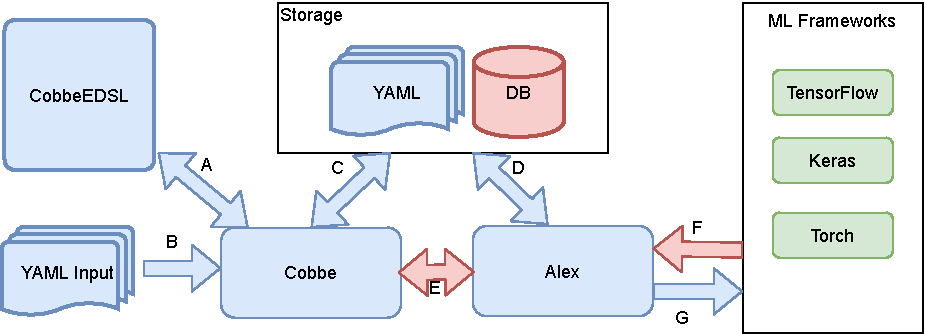
\includegraphics[width=\columnwidth]{pictures/framework_pic}
  \caption{This picture is not invisible}
\end{figure}


\section{An EDSL for construction of neural networks}




\section{Something about the venn diagram}


\section{Discussion}


\section{Future Work}



\begin{acks}
  acknowledgy stuff
\end{acks}

\bibliographystyle{ACM-Reference-Format}
\bibliography{bib}

\end{document}

%%% Local Variables:
%%% mode: latex
%%% TeX-master: t
%%% End:
